\documentclass{ledger}

%AUTHOR: This is a bare-bones template into which you may put your paper to aid in formatting your submission to Ledger. Note that to work properly, you must have the files "ledger.cls", "ledgerbib.bst", and the folder "images" on hand. 

%AUTHOR: the preferred method to generate PDF output is to use 'pdflatex'
%To clean up after a successful build, try: 'latexmk -c main.tex'

%EDITOR: in ledger.cls replace logoNewUC.png with logoNew.png prior to publication 


%EDITOR: replace X's to set the data for the header and footer
\newcommand{\thefirstpagenum}[0]{X}
\newcommand{\thelastpagenum}[0]{X}
\newcommand{\theyear}[0]{2024}
\newcommand{\thevol}[0]{X}
\newcommand{\thedoi}[0]{Asset Returns and Risk Projection}
\newcommand{\ledgerpages}[0]{\thefirstpagenum-\thelastpagenum}


\usepackage{paralist, caption}
\usepackage{booktabs} % For better table formatting
\usepackage{multirow} % For vertical centering across rows

\usepackage{tabularx}
\newcolumntype{Y}{>{\raggedleft\arraybackslash}X}
%\usepackage{siunitx} % For aligning numbers at the decimal point

%\usepackage[paperheight=16cm,paperwidth=12cm,textwidth=10cm]{geometry}

%AUTHOR: please set these to generate correct PDF metadata
\hypersetup{pdfauthor={iCapital Portfolio Analytics Quantitative Research Team}, pdftitle={Asset Returns and Risk Projection: Technical Manual}}

%EDITOR: set the correct pageination during layout
%\setcounter{page}{\thefirstpagenum}


%AUTHOR: this can be used to highlight changed text, surround with \edit{} and
%uncomment either to determine color
%\newcommand{\edit}[1]{{\color{red} #1}}
\newcommand{\edit}[1]{#1}
	
\overfullrule=10pt

\title{Asset Returns Projection}

\author{iCapital Portfolio Analytics Quantitative Research Team}

%\author{Firstname A. Lastname,\thanks{BTC/BCH/ETH ADDRESS}\thanks{F. A. Lastname (f.lastname@abc.edu) is a fictional author and researcher at the Centre for Blockchain Technology at the University of Central Wakanda, Birnin Zana, Wakanda} Firstname Q. Lastname,\thanks{F. Q. Lastname (firstname.lastname@businessname.ca) is  Director of Network Science at the Blockchain Center of Canadia.}}

\pagestyle{pagemain}


%The Author should select the appropriate pretitle below:
\pretitle{
  %\centering \selectfont LEDGER \LaTeX \ TEMPLATE \par
  %\centering \selectfont REVIEW ARTICLE \par
  %\centering \selectfont RESEARCH ARTICLE \par 
  %The Author should not remove the following text:
  \centering \large Technical Manual for \par 
  \fontsize{24pt}{28pt}\selectfont} % Title is centered and at 24pt


\begin{document}

\maketitle

\thispagestyle{pagefirst}

%\begin{abstract}
%Lorem ipsum dolor sit amet, consectetur adipiscing elit, sed do eiusmod tempor incididunt ut labore et dolore magna aliqua. Venenatis cras sed felis eget velit aliquet sagittis. Dis parturient montes nascetur ridiculus mus mauris vitae. Bibendum at varius vel pharetra vel. Amet mattis vulputate enim nulla aliquet porttitor. Urna porttitor rhoncus dolor purus non enim praesent elementum. Velit aliquet sagittis id consectetur purus ut faucibus pulvinar. Quam adipiscing vitae proin sagittis nisl rhoncus mattis rhoncus urna.\cite{Nakamoto2008} Risus quis varius quam quisque id. Habitasse platea dictumst quisque sagittis purus sit amet volutpat consequat.

%AUTHOR: keywords are OK to show for Review article, will be hidden and added to metadata for publication
%\begin{keywords}
%\item Lorem ipsum.
%\item Dolor.
%\item Sit amet.
%\end{keywords}
%\end{abstract}

\section{Introduction and Scope}
This project involves inputting historical asset class data to get return and risk projections for individual assets on Architect. We use Principal Components Regression to accomplish this task. There are two main inputs to this project:
\begin{compactenum}
	\item The historical returns of asset classes;
	\item The risk and return estimates provided by external CMA providers. \\
\end{compactenum}

\begin{figure}[!ht]
\centering
	%\captionsetup{justification=centering}
	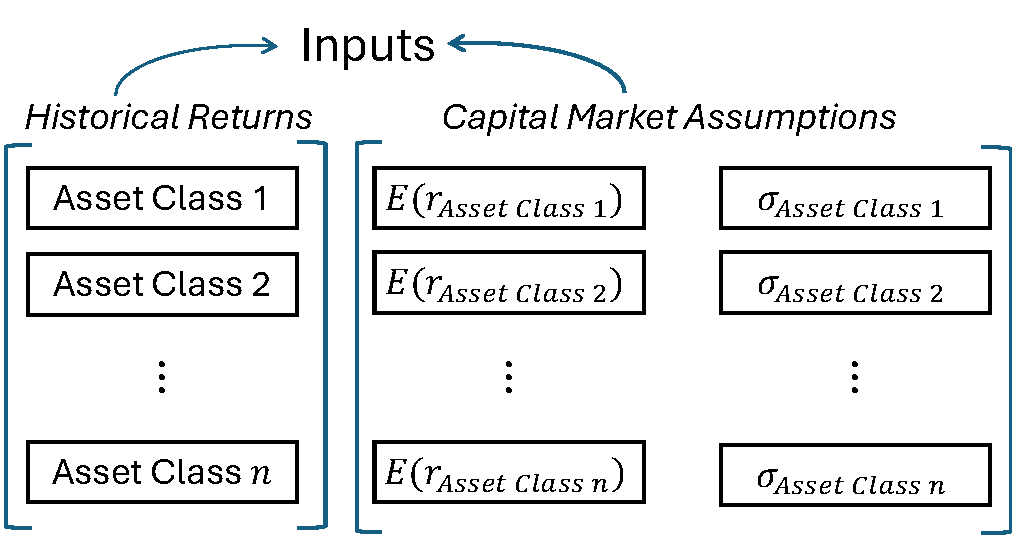
\includegraphics[width=250pt]{Inputs.pdf}
	 \caption{Inputs to the process.} ~\\
	%\label{graph1}
\end{figure}

The \textbf{outputs} to the process will be estimates of fund-level:
\begin{inparaenum}[$\bullet$]
	\item  future expected return;
	\item  and future expected risk
\end{inparaenum}
for each individual asset in Architect. We use \textbf{principal components regression (PCR)} to accomplish this task. 

\section{Methodology}
\begin{figure}[!ht]
\centering
	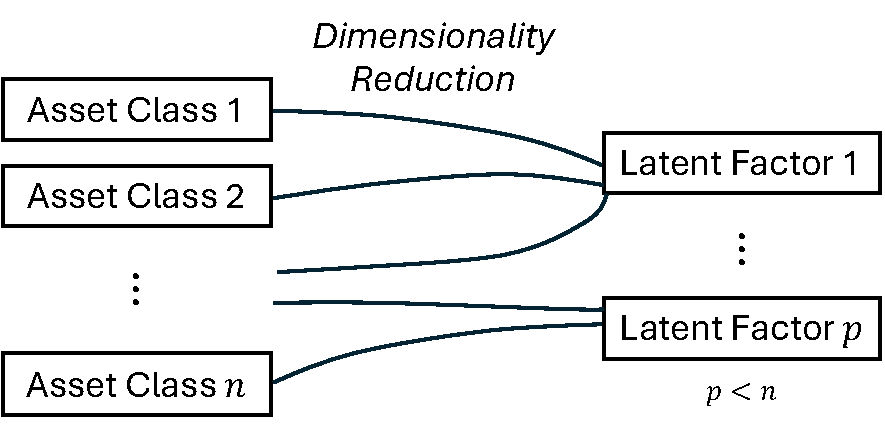
\includegraphics[width=225pt]{Step1.pdf}
	\caption{The first step in the methodology.} ~\\
\end{figure}

Principal components regression (PCR) is a technique used when the number of regressors is high, and are most likely correlated. Instead of regressing the dependent variable on all the explanatory variables, select principal components of the explanatory variables are used as regressors. One typically uses only a subset of all the principal components for regression; as a result, PCR could be interpreted as a kind of regularization procedure. It can also be vieiwed as a type of shrinkage estimator. \\

\begin{figure}[!ht]
\centering
	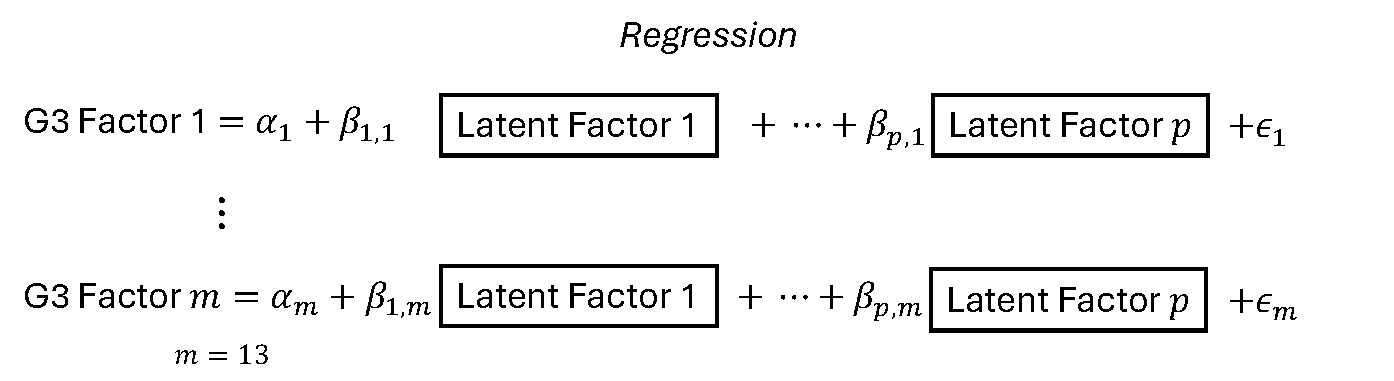
\includegraphics[width=375pt]{Step2.pdf}
	\caption{The second step in the methodology.} ~\\
\end{figure}

The basic methodology can be summed up in four steps. We do this for each of the 13 factors:
\begin{compactenum}
	\item Reduction of dimensionality of asset classes using principal components analysis.
	\item Coefficient generation on reduced feature set via ordinary least-squares regression; our factors on the left-hand-side (LHS), and the optimal reduced feature set (the components) on the right-hand-side (RHS). 
	\item Combine external CMAs with regression coefficients generated above to get future expected factor return and risk projections.  
	\item Use G3 factor loadings on future expected factor-projections to get asset-level projections. \\
\end{compactenum}

\begin{figure}[!ht]
\centering
	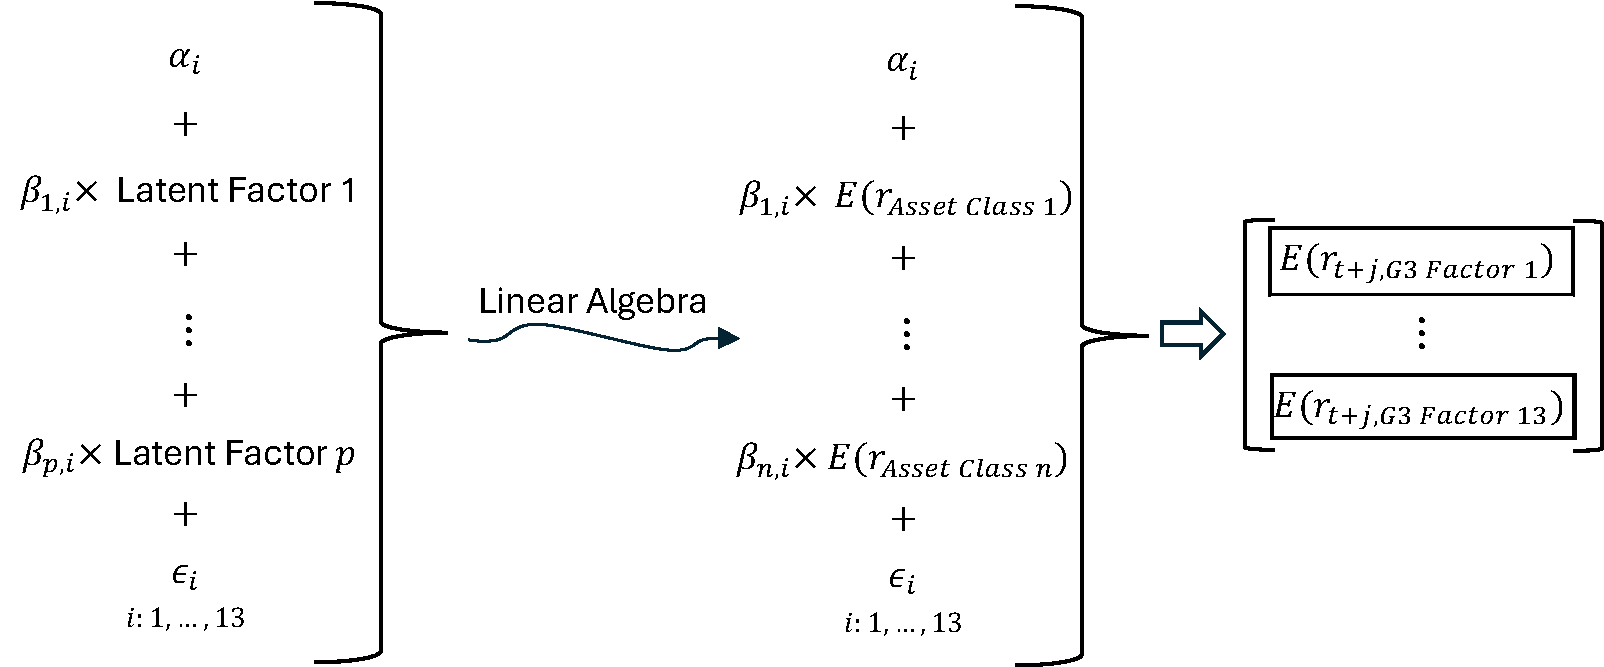
\includegraphics[width=375pt]{Step3.pdf}
	\caption{The third step in the methodology.} ~\\
\end{figure}

\subsection{Potential Issues and Solutions}

The principal components which have a higher percent-variance-explained (the ones based on eigenvectors corresponding to the higher eigenvalues of the sample variance-covariance matrix of the explanatory variables) are selected as regressors. It should be noted, however, that for the purpose of predicting the outcome, the principal components with lower percent-variance-explained may also be important\footnote{When Kendall and Hotelling first proposed PCR in the 1950s, they proposed ``complete" PCR, which means replacing the original variables by \textit{all} the principal components. Which principal components are included in the final model is determined by looking at the explained variance of the parameter estimates. By the early 1980s, the term PCR had changed to mean ``incomplete PCR.''}. The logic behind this is simple -- PCR does not consider the response variables (our factors) when deciding which components to drop; that decision is based only on the magnitude of the percent-variance-explained within the components themselves.\\

To resolve this, we use cross-validation to select the number of components to keep. So the overall methodology can be described as follows:
\begin{compactenum}
	\item Perform a 10-fold cross-validation baseline linear regression using all of the original independent variables (the original feature set). The mean of the cross-validation scores  from this regression is henceforth referred to as the  \textbf{\textit{baseline}} score. We use root mean square error (RMSE) for the cross-validation scores\footnote{Note that the number of folds, as well as the particular choice of score here is somewhat arbitrary. Other options were explored, and the results did not vary much. Also, we also used $R^2$ -- see Appendix for more details; the results did not change much.}.
	\item Perform a 10-fold cross-validation linear regression on each of the principal components. Use the mean of the cross-validation RMSEs for each component to compare with baseline.
	\begin{compactenum}[$\bullet$]	
		\item The number of principal components that minimize the difference between their own mean cross-validation score and the baseline RMSE are the optimal number of components required for the regression. 
	\end{compactenum}
	\item For each dependent variable in the regression (our factors), we then use the optimal number of components for that respective component. Also, for each dependent variable, we store: the coefficients, the error terms, and the intercept.
	\item We then use the Capital Market Assumptions to generate next-period return and risk measures for our factors, using the stored values above. \\
\end{compactenum}

In this manner, we ensure that, both:
\begin{compactenum}[$\bullet$]	
	\item the maximum variance of the independent variables; \textit{and}
	\item the explanatory power of the independent variables \textit{on} the dependent variables, 
\end{compactenum}
are accounted for. \\

\subsection{What is $k$-fold Cross-Validation?}

$k$-fold cross-validation is a widely used technique for assessing model performance. One splits the dataset into $k$ equal-sized subsets or folds. The model is then trained $k$ times, each time using $k-1$ folds for training and the remaining fold for testing. This process is repeated $k$ times, with each fold being used exactly once for testing. For time series, we must preserve the sequence of datapoints, so while we use all $k$ folds, it is done on an expanding-window basis. In other words, train on $k^{\text{th}}$ fold, and test on the $k+1^{\text{th}}$ fold. This process ensures that every data point is used for testing exactly once. After each training iteration, the model's performance is evaluated using the testing fold, typically by computing a performance metric which, in our case, is RMSE. The RMSEs from each iteration are then averaged to obtain a final performance metric for the model. Figure \ref{figure:cross_validation} below illustrates the process. \\

\begin{figure}[!ht]
\centering
	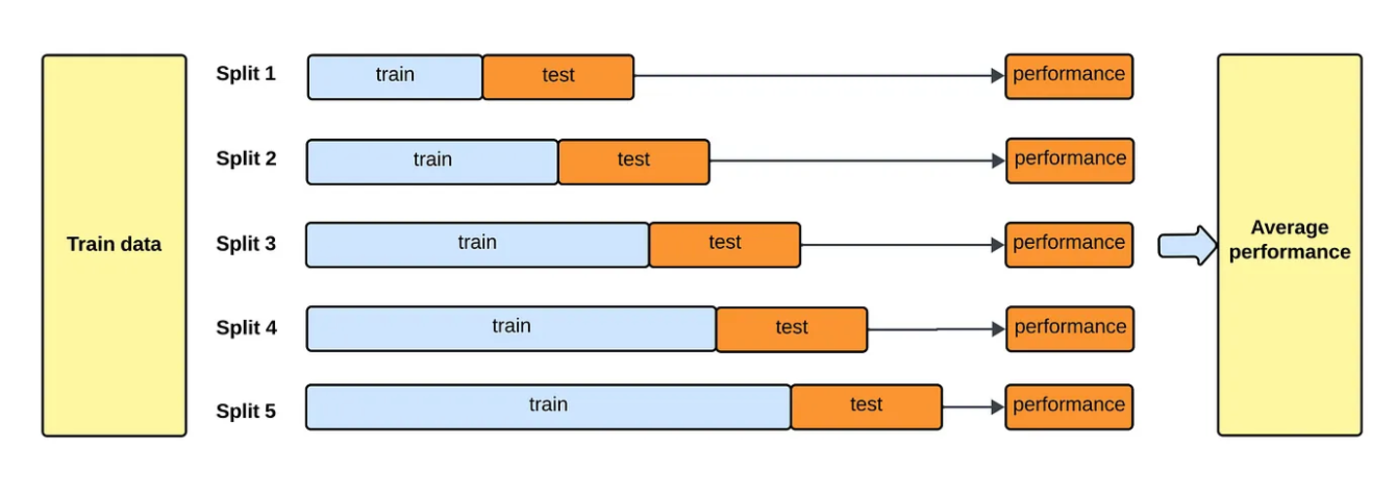
\includegraphics[width=375pt]{cross_validation_timeseries.pdf}
	\caption{An illustration of the cross-validation process for time series analysis.\label{figure:cross_validation}} ~\\
\end{figure}


$k$-fold cross-validation provides a more robust estimate of the model's performance compared to a single train-test split, as it evaluates the model on multiple subsets of the data. It also helps in detecting overfitting by assessing the model's generalization ability across different subsets of data\footnote{For documentation, the code used in the \texttt{KFold} function from the \texttt{scikit-learn} package, please refer to \href{https://scikit-learn.org/stable/modules/cross\_validation.html}{https://scikit-learn.org/stable/modules/cross\_validation.html}.}. \\

We also consider leave-one-out cross-validation (LOOCV), which is a special case of $k$-fold cross-validation. Here, $k$ is equal to the number of samples in the dataset. In LOOCV, the model is trained $k$ times, each time leaving out one sample for testing and training on the remaining samples. This process is repeated for each sample in the dataset, and the performance metrics are averaged across all iterations to obtain the final evaluation metric. \\

$k$-fold cross-validation strikes a balance between computational efficiency and robustness by dividing the dataset into smaller subsets, whereas LOOCV exhaustively trains the model on nearly all possible combinations of training and testing samples, making it computationally expensive for larger datasets. $k$-fold cross-validation provides a more efficient estimate of model performance and is more commonly used in practice. \\


\section{Results}

\subsection{Data}

The methodology in this paper was inspired by Haddad et al (2020)\footnote{Haddad, V., S. Kozak, S. Santosh. 2020. Factor Timing. \textit{The Review of Financial Studies}, 33(5):1980–2018.}. As we are still working on gathering asset class data, we use the public equity market anomaly dataset from Kozak et al. (2020)\footnote{Kozak, S., S. Nagel, and S. Santosh. 2020. Shrinking the cross-section. \textit{Journal of Financial Economics} 135:271–92.} as a placeholder for now. This dataset contains deciles of 54 equity market anomalies that effectively capture market heterogeneity. These anomalies are the usual anomalies like Size, Value, ROA, SUE, etc. The data already is broken up into deciles, and we create long-short portfolios for each anomaly (Decile 10 minus Decile 1) to emphasize the effects of each individual anomaly. The data is monthly and the months match our factor data from July 2004 to December 2019. Also, we break up the dataset into training and testing in an 80\%-20\% split, respectively. To preserve the temporal sequence, we do not shuffle the data before splitting it into the train and test set. \\

\subsection{Generating the Baseline RMSE}

We start with standardizing the original feature set. We do this by subtracting the mean, and dividing by the standard deviation. Note that the standardization is performed separately on the training and test set since means and standard deviations will differ across each portion. \\

We run a 10-fold cross-validation on the training set of the original (unmodified) features, to get a baseline RMSE. In other words, we are using the original feature set on the RHS to get a baseline RMSE. We also calculate the RMSE for the difference in predicted and actual values on the test set, using the parameter values generated from the test set. For the purposes of this project, we also ran lasso and ridge regressions for comparison. The results are shown in Table \ref{table:regression_rmse} below. \\

\begin{table}[ht]
\centering
\small % Adjust the font size 
\captionsetup{width=\textwidth, skip=4pt} % Adjust caption width and the space between the caption and the table
\caption{RMSE Results for Various Regression Techniques Across Different Dependent Variables. \label{table:regression_rmse}}
\begin{tabularx}{\textwidth}{>{\hsize=1.75\hsize}Y*{9}{>{\centering\arraybackslash\hsize=0.7\hsize}X}}
    \toprule
    & \multicolumn{3}{c}{\textbf{OLS}} & \multicolumn{3}{c}{\textbf{Lasso}} & \multicolumn{3}{c}{\textbf{Ridge}} \\
    \cmidrule(lr){2-4} \cmidrule(lr){5-7} \cmidrule(lr){8-10}
    \multirow{-2.5}{*}{\textbf{Dependent Var}} & {\textbf{Train}} & {\textbf{Test}} & {\textbf{\%$\Delta$}} & {\textbf{Train}} & {\textbf{Test}} & {\textbf{\%$\Delta$}} & {\textbf{Train}} & {\textbf{Test}} & {\textbf{\%$\Delta$}} \\
    \midrule
    Alt Commodities & 7.65 & 5.51 & -27.93 & 5.12 & 2.27 & -55.77 & 6.39 & 4.36 & -31.75 \\
    Alt HF Crowding & 5.08 & 3.83 & -24.61 & 3.69 & 3.11 & -15.64 & 4.25 & 3.44 & -19.21 \\
    Alt Oil & 11.64 & 9.58 & -17.70 & 8.10 & 6.79 & -16.23 & 9.69 & 8.41 & -13.19 \\
    Alt Trend & 3.66 & 4.23 & 15.64 & 2.82 & 2.84 & 0.85 & 3.17 & 3.60 & 13.53 \\
    Emerging Mkts & 9.85 & 8.38 & -14.92 & 7.12 & 4.53 & -36.44 & 8.19 & 6.46 & -21.19 \\
    Equity Market & 5.96 & 5.92 & -0.71 & 4.66 & 3.26 & -30.07 & 5.09 & 4.69 & -7.85 \\
    Momentum & 5.86 & 4.73 & -19.29 & 4.29 & 2.76 & -35.66 & 4.93 & 3.64 & -26.06 \\
    Equity Quality & 3.07 & 2.53 & -17.46 & 2.31 & 1.85 & -20.20 & 2.69 & 2.28 & -15.30 \\
    Equity SmallCap & 3.58 & 3.35 & -6.25 & 2.73 & 2.24 & -18.09 & 3.07 & 2.91 & -5.46 \\
    Equity Value & 1.33 & 1.70 & 27.39 & 0.98 & 1.44 & 46.90 & 1.14 & 1.57 & 38.02 \\
    Fixed Credit & 4.17 & 2.52 & -39.58 & 2.85 & 1.21 & -57.52 & 3.50 & 1.94 & -44.37 \\
    Fixed Duration & 2.41 & 2.06 & -14.38 & 1.82 & 1.46 & -19.61 & 2.02 & 1.71 & -15.30 \\
    US Dollar & 3.62 & 2.60 & -28.24 & 2.49 & 1.61 & -35.15 & 2.99 & 2.19 & -26.76 \\
    \bottomrule \\
\end{tabularx}
\end{table}

Notably, Alt Trend has an \textit{increase} in RMSE from the training to the test set\footnote{On a separate note, when running a stepwise regression, none of the independent variables showed significance for this factor, so these variables have limited predictive power for this factor.}. The same is seen for Equity Value. Otherwise, we see a good reduction in RMSE from the training to the test set, which is validation for our technique. \\

Note that the Lasso and ridge regressions were run only for control purposes. We will use the RMSE from the training set of the OLS as a baseline RMSE. The logic behind this is to use the original features on the training data to get a baseline. \\

\subsection{Principal Components Regression}

We now run PCA on the training part of the RHS dataset, and store all the components. Next, we run OLS, with cross-validation, using each of the components one-by-one on the RHS, and with the each factor on the LHS. To clarify what is done here, we use the train-part of the 80-20 train-test split performed above. On this part, we take each factor (say, Alt Commodities to start), and put it on the LHS. Next, we run as many OLS regressions as there are components, adding components one-by-one, and performing a 10-fold cross-validation for each regression, for each component. For each component we then get an average RMSE (across all cross-validations), which we will compare with the baseline RMSE calculated from the cross-validated regression run above using the original features. For each factor, we get a result that looks like Figure \ref{figure:fixed_duration_cv_pca}. The results for the other factors are summarized in the Table \ref{table:summary_cv_scores} below. \\

\begin{figure}[!ht]
\centering
	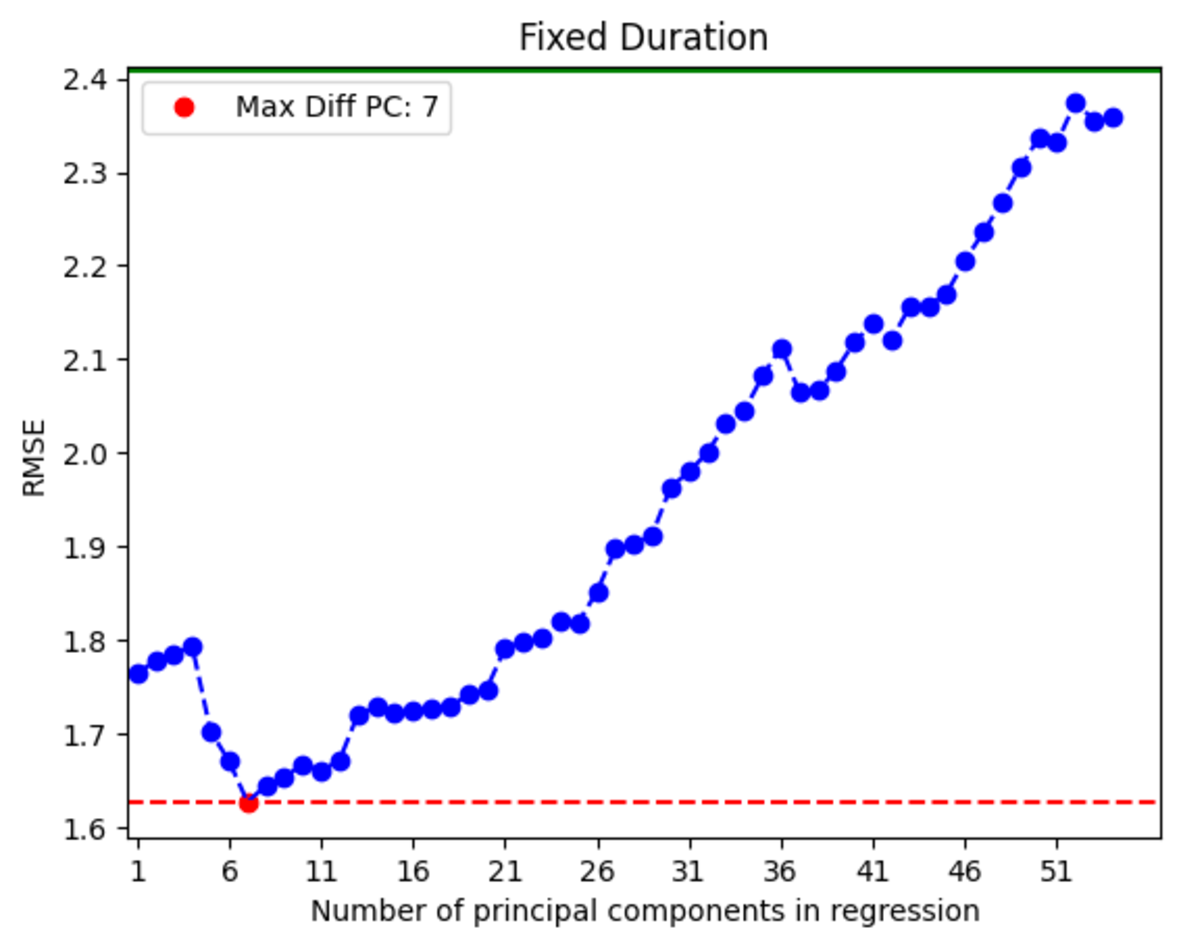
\includegraphics[width=300pt]{FixedDuration_CV_PCA.pdf}
	\caption{The results of running cross-validation on each principal component one-by-one on the Fixed Duration factor. In this case, the RMSE is minimized on the seventh principal component compared to the baseline. \label{figure:fixed_duration_cv_pca}} ~\\
\end{figure}

\begin{table}[!ht]
	\centering
	\caption{CV Scores with Optimal PC Count from PCR.}
	\label{table:summary_cv_scores}
	\begin{tabularx}{350pt}{rcccc}
	\toprule
		\textbf{Dependent Variable} & \textbf{Components} & \textbf{Train RMSE} & \textbf{Test RMSE} & \textbf{\% Diff} \\
	\midrule
		Alt Commodities & 1 & 5.03 & 2.34 & -53.55\% \\
		Alt HF Crowding & 1 & 3.53 & 3.32 & -5.84\% \\
		Alt Oil & 1 & 8.06 & 7.00 & -13.12\% \\
		Alt Trend & 1 & 2.78 & 2.85 & 2.72\% \\
		Emerging Markets & 1 & 6.97 & 4.42 & -36.59\% \\
		Equity Market & 1 & 4.29 & 3.67 & -14.58\% \\
		Equity Momentum & 1 & 4.12 & 2.73 & -33.62\% \\
		Equity Quality & 1 & 2.16 & 1.87 & -13.28\% \\
		Equity SmallCap & 1 & 2.63 & 2.32 & -11.63\% \\
		Equity Value & 1 & 0.95 & 1.44 & 52.01\% \\
		Fixed Credit & 1 & 2.52 & 1.45 & -42.64\% \\
		Fixed Duration & 7 & 1.63 & 1.46 & -10.45\% \\
		US Dollar & 1 & 2.37 & 1.62 & -31.71\% \\
	\bottomrule \\
	\end{tabularx} 
\end{table} 

\subsection{Calculating Factor Expected Returns}
The final step in the project is to calculate factor expected returns. We will use the asset class expected returns provided by external CMA providers for this. For now, we use the anomaly dataset historical returns. \\

\subsubsection{Issues and Solution} 
It's important to note that we are using the coefficients from the regression run after two modifications on the original feature set, i.e., the asset classes: \begin{inparaenum}[(i)] \item standardization or normalization; and \item principal components analysis.\end{inparaenum}We will be using the returns provided by the external CMA providers, along with the coefficients and intercept from the PCR. These externally-provided returns are the 10-year projections of the original feature set. We must somehow find a way to adjust the coefficients so that they match up with the original feature set, and not the standardized feature set in ``principal components space''\footnote{Recall that principal components analysis transforms the original features into a new set of orthogonal features, capturing maximum variance in a lower-dimensional space.}. To do this, we rely on the equivalence between PCA and singular value decomposition. Please see the Appendix for details on the methodology used and the corresponding linear algebra. \\

\subsubsection{Final Results}
Table \ref{table:projection_vs_actual} shows the projections and the historical means of the factor returns across the entire time period (July 2004 to December 2019). Data has been left as monthly here for factual clarity, but should be annualized in the final version of the implementation\footnote{Historical means for the anomalies were also used in place of externally-provided CMAs here.}. \\

\begin{table}[ht]
\centering
\caption{Comparison of Projection and Historical Means for Factors. \label{table:projection_vs_actual}}
	\begin{tabularx}{300pt}{rccc}
	\toprule
		\textbf{Factor} & \textbf{Projection} & \textbf{Historical Mean} & \textbf{Difference} \\
	\midrule
		Alt Commodities & -0.0026 & -0.0025 & -0.00002 \\
		Alt HF Crowding & 0.0062 & 0.0045 & 0.0017 \\
		Alt Oil & 0.0060 & 0.0067 & -0.0007 \\
		Alt Trend & 0.0058 & 0.0040 & 0.0017 \\
		Emerging Markets & 0.0061 & 0.0039 & 0.0022 \\
		Equity Market & 0.0048 & 0.0054 & -0.0006 \\
		Equity Momentum & 0.0049 & 0.0053 & -0.0003 \\
		Equity Quality & 0.0034 & 0.0037 & -0.0003 \\
		Equity SmallCap & 0.0028 & 0.0017 & 0.0011 \\
		Equity Value & -0.0012 & -0.0017 & 0.0005 \\
		Fixed Credit & 0.0053 & 0.0050 & 0.0004 \\
		Fixed Duration & 0.0038 & 0.0031 & 0.0006 \\
		US Dollar & 0.0007 & 0.0007 & -0.00003 \\
	\bottomrule
	\end{tabularx}
\end{table}

\section{Conclusion and Further Research}
We applied Principal Components Regression (PCR) coupled with cross-validation to generate projections for our factor set. By utilizing PCR, we optimally reduced the dimensionality of our dataset, enabling us to focus on the most significant components, minimize multicollinearity, and enhance predictive power. Our approach involved standardizing the feature set, applying PCA for dimensionality reduction, using cross-validation for optimal principal component choice\footnote{One idea that is under development is using LARS (least angle regression) LASSO instead of OLS like we do currently for calculating the optimal number of PCs.}, and then fitting linear regression models to the transformed data. \\

We assessed model performance using both, $R^2$ and RMSE metrics through $k$-fold and leave-one-out cross-validation strategies. This allowed us to fine-tune the number of principal components, balancing model simplicity with predictive accuracy. The results highlight PCR's utility in extracting meaningful insights from complex datasets, offering a streamlined yet powerful model for predicting factor behaviors. \\

The findings underscore the potential of PCR in enhancing decision-making in multiple areas of alternative investment management, providing a scalable and interpretable framework for predictive modeling. \\

Next steps involve:
\begin{compactenum}[$\bullet$]	
	\item Implementing G3 de-smoothing to convert quarterly asset class returns to monthly; 
	\item Using G3 factor loadings to project out asset-level returns; and
	\item Devising a technique for covariance matrix projection.
\end{compactenum}

\newpage

%define the following sections to hide their Section Number (Notes Style)
\ledgernotes
\section*{Appendix}

\section*{\normalsize \textit{Linear Algebra for ``Converting'' PCR Coefficients}}

Let $R_{T \times N}$ be the historical returns of $N$ indices corresponding to CMA asset classes for $T$ periods. Using Singular Value Decomposition (SVD):
\begin{equation}
	R_{T \times N} = U_{T \times T} \Sigma_{T \times N} V_{N \times N}^{T}
\end{equation}
where $U$, $V$ are the left and right orthonormal eigenvectors and $\Sigma$ has the singular values along its diagonal. We may reduce the dimensionality by limiting to the first $K$ eigenvalues (principal components):
\begin{equation} 
	R_{T \times N} \approx U_{T \times K} \Sigma_{K \times K} V_{K \times N}^{T} = X_{T \times K} V_{K \times N}^{T} 
\end{equation}

Let $F_{T \times P}$ be the historical returns of $P$ risk factors, we can propose a linear relationship between the factors and the CMAs as:
\begin{equation} 
	F_{T \times P} = R_{T \times N} \beta_{N \times P}^{T} \approx X_{T \times K} V_{K \times N}^{T} \beta_{N \times P}^{T} = X_{T \times K} \beta_{K \times P}^{T} 
\end{equation}

So we can estimate $\beta_{K \times P}^{\prime} = f(F_{T \times P}, X_{T \times K})$. From the above equations we have --
\begin{equation} r_{N} \approx V_{N \times K} x_{K} \end{equation}
\begin{equation} f_{P} \approx \beta_{P \times K} x_{K} \approx B_{P \times K} V_{K \times N}^{T} r_{N} \end{equation}
Thus, given a vector of projected returns for the CMAs $r_{N}$, we can estimate a vector of projected returns for risk factors $f_{P}$.

\newpage

\section*{\normalsize \textit{Using $R^2$ instead of RMSE}}
The results are somewhat consistent with using RMSE. It is concerning that the $R^2$ values are all negative, indicating underperformance to a standard mean model. It may be worthwhile to explore running a partial least squares or LARS LASSO instead of a principal components regression. However, this could just be an issue with the anomaly dataset. \\

\begin{table}[!ht]
\centering
	\caption{R\(^2\) Scores for Various Models. \label{table:r2_scores}}
	\begin{tabularx}{\textwidth}{l *{6}{X}}
	\toprule
		\textbf{Dependent Variable} & \multicolumn{2}{c}{\textbf{OLS}} & \multicolumn{2}{c}{\textbf{Lasso}} & \multicolumn{2}{c}{\textbf{Ridge}} \\
	\cmidrule(lr){2-3} \cmidrule(lr){4-5} \cmidrule(lr){6-7}
		& \textbf{Train} & \textbf{Test} & \textbf{Train} & \textbf{Test} & \textbf{Train} & \textbf{Test} \\
	\midrule
		Alt Commodities & -1.55 & -4.92 & -0.12 & -0.00 & -0.80 & -2.71 \\
		Alt HF Crowding & -1.55 & -0.53 & -0.10 & -0.01 & -0.74 & -0.23 \\
		Alt Oil & -0.97 & -0.99 & -0.02 & -0.00 & -0.39 & -0.54 \\
		Alt Trend & -0.92 & -1.43 & -0.09 & -0.10 & -0.44 & -0.76 \\
		Emerging Markets & -1.18 & -2.63 & -0.05 & -0.06 & -0.47 & -1.15 \\
		Equity Market & -1.01 & -2.48 & -0.15 & -0.06 & -0.45 & -1.19 \\
		Equity Momentum & -1.31 & -1.94 & -0.15 & -0.00 & -0.63 & -0.75 \\
		Equity Quality & -1.03 & -0.94 & -0.09 & -0.03 & -0.57 & -0.57 \\
		Equity SmallCap & -1.27 & -1.39 & -0.08 & -0.06 & -0.58 & -0.79 \\
		Equity Value & -1.13 & -0.40 & -0.09 & -0.00 & -0.52 & -0.20 \\
		Fixed Credit & -2.21 & -3.95 & -0.14 & -0.14 & -1.18 & -1.96 \\
		Fixed Duration & -1.18 & -1.05 & -0.17 & -0.03 & -0.50 & -0.40 \\
		US Dollar & -1.33 & -1.60 & -0.10 & -0.00 & -0.63 & -0.85 \\
	\bottomrule \\
	\end{tabularx} 
\end{table}

\begin{figure}[!ht]
\centering
	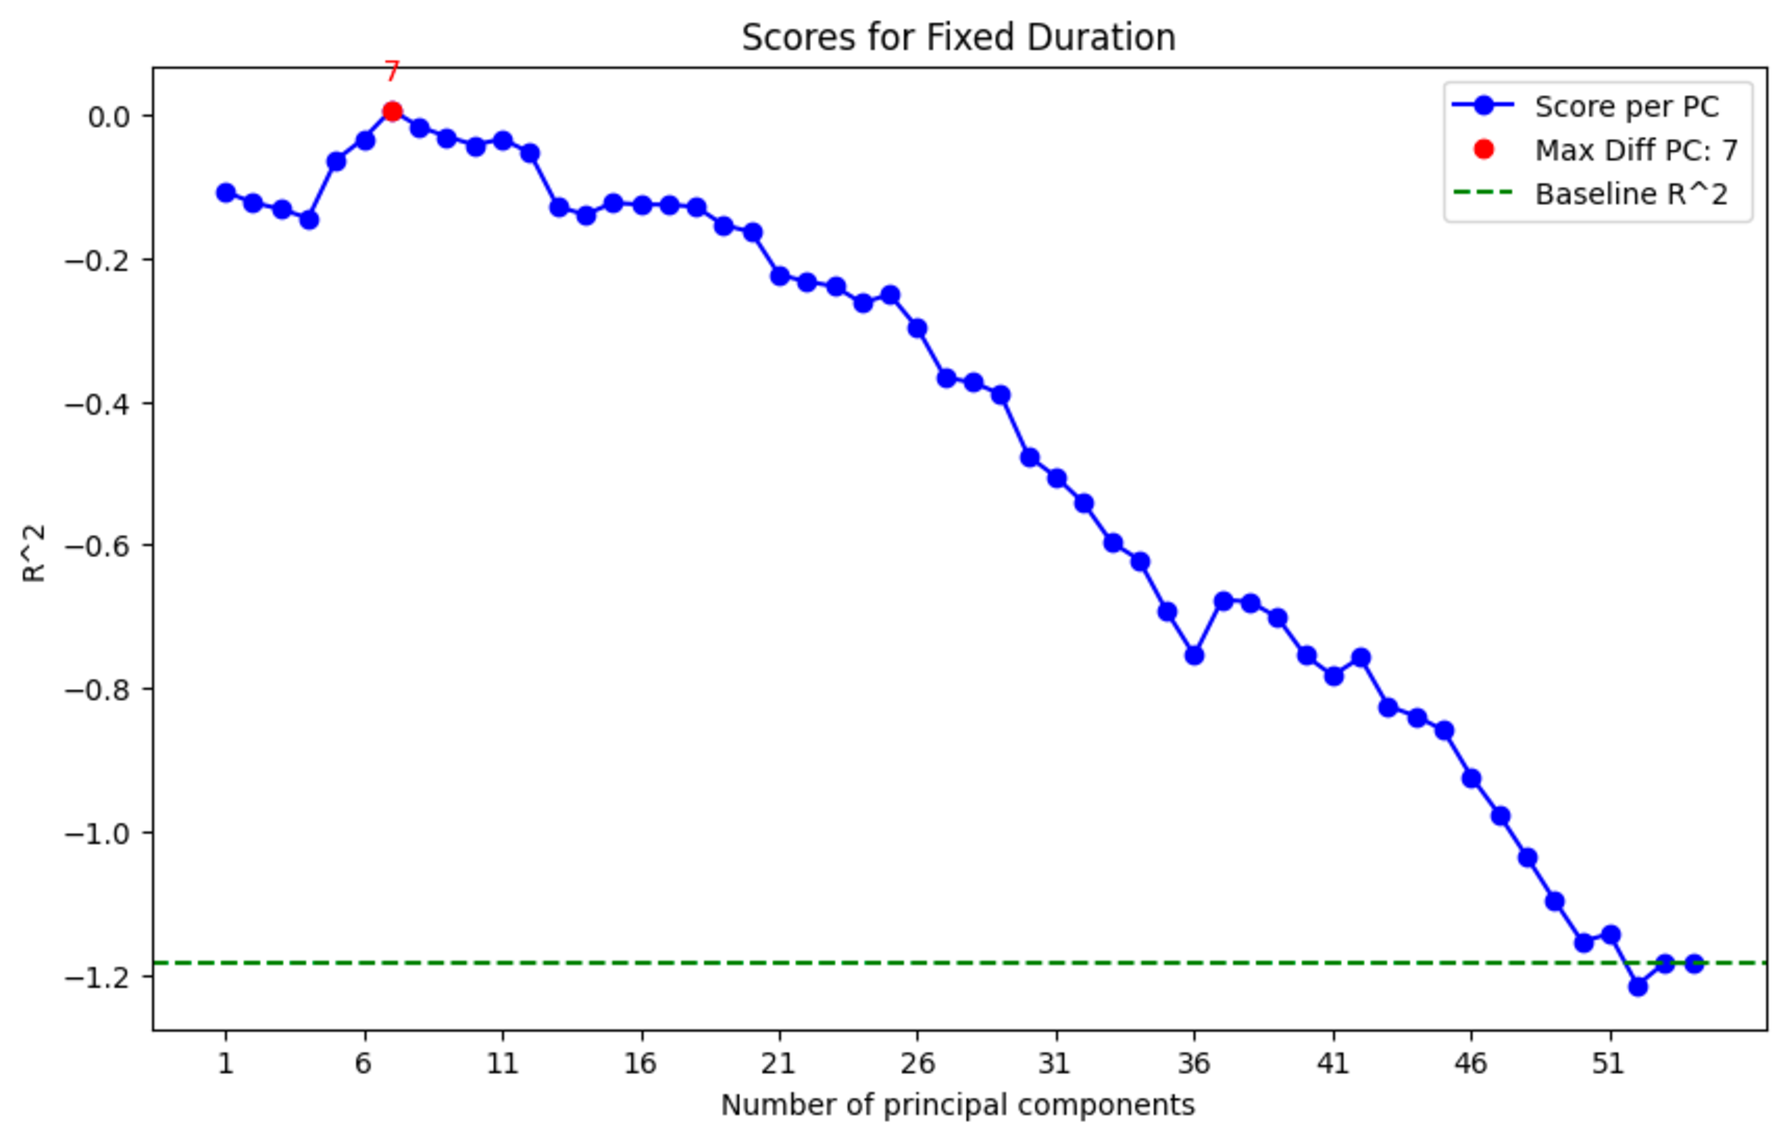
\includegraphics[width=325pt]{FixedDuration_CV_PCA_R2.pdf}
	\caption{The results of running cross-validation on each principal component one-by-one on the Fixed Duration factor. In this case, the $R^2$ is maximized on the seventh principal component compared to the baseline. The results are consistent with using RMSE. \label{figure:fixed_duration_cv_pca_r2}} ~\\
\end{figure}

\newpage

\section*{\normalsize \textit{Using Leave-One-Out (LOO) instead of $k$-Fold Cross-Validation}}
The final out-of-sample PCR results are consistent with using $k$-fold cross-validation, but the computation time increases significantly ($\sim$ 12x). Interestingly, the optimal principal component count for Alt HF Crowding and Fixed Credit change. \\

\begin{table}[!ht]
	\centering
	\caption{LOO Cross Validation RMSE Scores. \label{table:loo_cross_validation}}
	\begin{tabularx}{\textwidth}{l *{9}{X}}
	\toprule
		\textbf{Dependent Variable} & \multicolumn{3}{c}{\textbf{OLS}} & \multicolumn{3}{c}{\textbf{Lasso}} & \multicolumn{3}{c}{\textbf{Ridge}} \\
	\cmidrule(lr){2-4} \cmidrule(lr){5-7} \cmidrule(lr){8-10}
			& \textbf{Train} & \textbf{Test} & \textbf{\% $\Delta$} & \textbf{Train} & \textbf{Test} & \textbf{\% $\Delta$} & \textbf{Train} & \textbf{Test} & \textbf{\% $\Delta$} \\
	\midrule
		Alt Commodities & 6.49 & 5.51 & -15.08 & 5.18 & 2.27 & -56.23 & 5.71 & 4.36 & -23.57 \\
		Alt HF Crowding & 4.95 & 3.83 & -22.53 & 3.65 & 3.11 & -14.65 & 4.18 & 3.44 & -17.89 \\
		Alt Oil & 10.26 & 9.58 & -6.65 & 8.06 & 6.79 & -15.80 & 9.01 & 8.41 & -6.58 \\
		Alt Trend & 3.68 & 4.23 & 15.12 & 2.82 & 2.84 & 0.70 & 3.21 & 3.60 & 12.29 \\
		Emerging Markets & 8.99 & 8.38 & -6.72 & 7.14 & 4.53 & -36.61 & 7.83 & 6.46 & -17.50 \\
		Equity Market & 5.15 & 5.92 & 14.91 & 4.76 & 3.26 & -31.45 & 4.75 & 4.69 & -1.16 \\
		Equity Momentum & 5.48 & 4.73 & -13.69 & 4.28 & 2.76 & -35.53 & 4.77 & 3.64 & -23.61 \\
		Equity Quality & 2.68 & 2.53 & -5.56 & 2.30 & 1.85 & -19.68 & 2.48 & 2.28 & -8.27 \\
		Equity SmallCap & 3.31 & 3.35 & 1.21 & 2.72 & 2.24 & -17.91 & 2.99 & 2.91 & -2.82 \\
		Equity Value & 1.29 & 1.70 & 31.64 & 0.98 & 1.44 & 47.06 & 1.12 & 1.57 & 40.94 \\
		Fixed Credit & 3.73 & 2.52 & -32.42 & 2.79 & 1.21 & -56.72 & 3.30 & 1.94 & -41.00 \\
		Fixed Duration & 2.41 & 2.06 & -14.33 & 1.86 & 1.46 & -21.34 & 2.06 & 1.71 & -17.29 \\
		US Dollar & 3.16 & 2.60 & -17.61 & 2.43 & 1.61 & -33.47 & 2.79 & 2.19 & -21.36 \\
	\bottomrule \\
	\end{tabularx}
\end{table}

\begin{table}[ht]
\centering
\caption{RMSE Scores from PCR with Optimal PC Count Using LOO Cross-Validation are Consistent with $k$-Fold. \label{table:rmse_scores_LOO}}
	\begin{tabularx}{350pt}{lcccr}
	\toprule
		\textbf{Dependent Variable} & \textbf{Components} & \textbf{Train RMSE} & \textbf{Test RMSE} & \textbf{\% Diff} \\
	\midrule
		Alt Commodities & 1 & 0.0502 & 0.0234 & -53.50\% \\
		Alt HF Crowding & 12 & 0.0326 & 0.0320 & -1.88\% \\
		Alt Oil & 1 & 0.0810 & 0.0700 & -13.48\% \\
		Alt Trend & 1 & 0.0280 & 0.0285 & 1.81\% \\
		Emerging Markets & 1 & 0.0696 & 0.0442 & -36.57\% \\
		Equity Market & 1 & 0.0435 & 0.0367 & -15.66\% \\
		Equity Momentum & 1 & 0.0419 & 0.0273 & -34.73\% \\
		Equity Quality & 1 & 0.0215 & 0.0187 & -13.00\% \\
		Equity SmallCap & 1 & 0.0265 & 0.0232 & -12.27\% \\
		Equity Value & 1 & 0.0095 & 0.0144 & 52.72\% \\
		Fixed Credit & 2 & 0.0266 & 0.0146 & -45.26\% \\
		Fixed Duration & 7 & 0.0158 & 0.0146 & -7.62\% \\
		US Dollar & 1 & 0.0240 & 0.0162 & -32.48\% \\
\bottomrule
\end{tabularx}
\end{table}

%define the following sections to hide their Section Number (Notes Style)
%\ledgernotes

%\section*{Acknowledgements} 
%
%FAL and FQL thank Fancy Scholar for his 
%invaluable comments on several drafts of this paper. 
%FAL acknowledges the University of Central Wakanda for their financial support.

% \section*{Author Contributions}

% State the contribution made by each author.  Refer to authors using their initials, for example, ``FAL developed the code to perform the simulation (65\%) and FQL analyzed the results (35\%).  They both contributed equally to manuscript preparation.''

% \section*{Conflict of Interest}

% Authors should state any conflict of interest as defined by Ledger's Conflict of Interest Policy, available on the Ledger website. If the author believes there are no conflicts of interest, they should include the following: ``The author declares that they have no known conflicts of interest as per the journal’s Conflict of Interest Policy.''

%AUTHOR: comment out if using thebibliography
%\theendnotes

%AUTHOR: please read ledgerbib.bst usage notes by opening it in a text editor. We have modified it to include the use of the @misc item type for the proper formatting of online sources.

\newpage

\bibliographystyle{ledgerbib}
\bibliography{FactorReturnsProjection}
\nocite{*}


%AUTHOR: comment out, this is used to make sure the Creative Commons License
%image fits on page

\newpage

%define the following sections to have the Appendix Style

%\appendix
%\setcounter{section}{0}
%\section{Data and Descriptions}





%\newpage
%here up^^


\thispagestyle{pagelast}





%\theendnotes

\end{document}
